\chapter[Préparation des données]{Préparation des données}
\label{dataprepation}
\chapterabstract
{
Dans ce chapitre nous allons expliciter les différentes étapes abordées dans la préparation des données utilisés dans ce travail, comme l’extraction des données à partir des prévisions du modèle de prévision numérique du temps (AROME, modèle opérationnel à la Direction de la Météorologie Nationale), les transformations des données et la construction de la base de données finale. Vers la fin de ce chapitre, nous allons expliquer l'approche adoptée pour la répartition et l’échantillonnage de ces données en deux fichiers (test et apprentissage) afin de garantir la représentativité des mois, des heures et des diverses classes de visibilités pour toutes les stations synoptiques.
}
\pagestyle{plain}

La préparation des données consiste à transformer les données brutes en des ressources d'information compréhensible et affinées. C'est une étape fondamentale de l'analyse des données en général et du Datamining en particulier. Cette activité comprend plusieurs tâches à savoir l'acquisition et le chargement des données, contrôle de la qualité des données, et la transformation des données lorsqu'il le faut. \\

Le jeu de données utilisées dans ce travail est déjà préparé dans une étude réalisée à la Direction de la Météorologie Marocaine par \citep{Ouagabi-Bari2018}. Dans ce qui suit, nous allons présenter brièvement les grandes phases de préparation des données, ainsi que la configuration de l'échantillonnage adoptée au cours de ce travail (Cf. Fig. \ref{rep_donnees}).\\

La base de données utilisée dans ce travail couvre les données horaires de 3 ans (2014, 2015 et 2016), résultat d’un prétraitement des sortie brutes du modèle de prévision numérique AROME et des données observées.\\

\begin{tcolorbox}
\footnotesize {
Le modèle non-hydrostatique AROME \citep{seity2011arome} est le modèle de prévision numérique du temps à maille fine exploité en opérationnel à la Direction de la Météorologie Nationale. Il a été conçu pour améliorer la prévision à courte échéance des phénomènes dangereux tels que les fortes pluies méditerranéennes, les orages violents, le brouillard ou les îlots de chaleur urbains en période de canicule. Il a été développé grâce à d’étroites collaborations, nationales et internationales, afin de tenir compte des dernières avancées en modélisation atmosphérique.
}
\end{tcolorbox}

Les fichiers de données brutes issues des prévisions d’AROME sont considérés comme les fichiers en entrée du package FullPos.

\begin{tcolorbox}
\footnotesize {
FullPos est un package de post-traitement puissant et sophistiqué. Il est destiné à être utilisé pour l'exploitation et la recherche. FullPos a deux parties principales : les interpolations verticales, puis les interpolations horizontales. Entre les deux, un traitement spectral est parfois possible pour les champs dynamiques.
}
\end{tcolorbox}

Ci-dessous les grandes étapes qui sont établis au cours de préparation et de traitement des sorties du modèle AROME:
\begin{enumerate}
    \item Application du FullPOS sur les fichiers bruts de prévision en format LFI par jour et par échéance ;
    \item Extraction des 29 paramètres météorologiques qui seront utilisés comme prédicteurs par date, heure, latitude et longitude de chaque point de grille du domaine d’étude ;
    \item Extraction des lignes correspondantes aux points de grille le plus proche de chaque station
synoptique du domaine d’étude ;
    \item Transformation des données générées au format adéquat à l’utilisation lors de la phase de
modélisation et génération de la direction et de la vitesse du vent à partir des composantes
zonale et méridionale du vent ;
\end{enumerate}

\section{Traitement des sorties brutes du modèle AROME}
\ding{109} L’extraction des sorties du modèle de prévision numérique du temps (PNT) a été réalisé par un script développé à base du FullPoss, avec une durée d’une semaine sur le super calculateur IBM de Maroc Météo. Ainsi, une conversion en format ASCII a été établi sur les données stocké dans les fichiers FullPoss de taille 128 mo/fichier. Ainsi, la taille globale a atteint 128 mo/fichier x 24 fichier/jour x 365 jours/an x 3 ans = 3363840 mo= 3.36To). \\

\ding{109} Transformation des données inclut le calcul de nouveaux champs ainsi la conversion des unités de mesure pour quelques variables comme il est présenté dans la table \ref{tabl_trans}.
\begin{table}[ht]
\begin{center}
\begin{tabular}{ |c|c|c| } 
\hline
\textbf{Variable} & \textbf{transformation} & \textbf{équation} \\
\hline
CLSTEMPERATURE & Kelvin -> \degree C & CLSTEMPERATURE-273.15\\
\hline
CLSHUMI.RELATIVE & Décimale -> \% & CLSHUMI.RELATIVEx100\\
\hline
MSLPRESSURE & Bar -> millibar & MSLPRESSURE/100\\
\hline
H00010TEMPERATUR & Kelvin -> \degree C & H00010TEMPERATUR-273.15\\
\hline
H00010HUMI\_RELAT & Décimale -> \% & H00010HUMI\_RELATx100\\
\hline
H00010TEMPE\_POTE & Kelvin -> \degree C & H00010TEMPE\_POTE-273.15\\
\hline
H00010THETA\_PRIM & Kelvin -> \degree C & H00010THETA\_PRIM-273.15\\
\hline
H00010PRESSURE & Bar -> millibar & H00010PRESSURE/100\\
\hline
SURFPRESSION & Bar -> millibar & SURFPRESSION/100\\
\hline
\end{tabular}
\caption{Les transformation sur les champs des sorties du modèle PNT}\label{tabl_trans}
\end{center}
\end{table}

\section{Traitement des données observées brutes}
Les données météorologiques utilisées dans cette étude sont extraites des Comptes Rendus Quotidiens
(CRQ) issus de chacune des stations synoptiques incluses dans la zone d’étude, et regroupée tous dans
un fichier texte. Ainsi, un prétraitement a été établi sur ces données afin de:
\begin{itemize}
    \item[\ding{230}] Supprimer les lignes avec données manquantes en visibilité.
    \item[\ding{230}] Supprimer des lignes avec des données aberrantes en visibilité (valeurs qui dépassent
30000m)
    \item[\ding{230}] Extraire des données issues des stations faisant partie du domaine (longitude entre -0.045 et
-10.295 ; latitude entre 28.64 et 37.84) et de la période d’étude.
\end{itemize}

\section{Préparer la base de données finale}
Après l'extraction et les transformations des donnée, la phase de la fusion des données dans un fichier final a été effectuée. Voici les étapes suivies pour fusionner ces données: 
\begin{enumerate}
    \item Extraire les données météorologiques observées correspondantes à la première station;
    \item Extraire les prévisions du modèle AROME correspondants au point de grille le plus proche à la
première station;
    \item Fusionner les deux ensembles de données qu’on vient d’extraire par jointure en passant la date
et l’heure comme clé de cette jointure, incluant tous les paramètres du modèle AROME, et
seulement la visibilité observée à partir des données météorologiques;
    \item Insérer le résultat de cette jointure dans un fichier de données final;
    \item Refaire le même processus pour les autres stations, et les rassembler toutes dans un fichier final.
\end{enumerate}
\section{Échantillonnage des données en sous-ensembles d'apprentissage et de test}
le fichier final, construit le jeu de données de notre étude, a été subdivisé en:\\

\begin{itemize}
    \item[\ding{230}] \textbf{Fichier d’apprentissage} : permet au modèle développé d’apprendre et de s’adapter par comparaison entre le résultat qu’il calcule en fonction des entrées fournies, et la réponse attendue en sortie. La taille de ce fichier dans ce travail constitue 70\% du fichier final;\\
    
    \item[\ding{230}] \textbf{Fichier de test} : contient des données indépendantes du fichier d’apprentissage et permet de tester la performance du modèle développé. La taille de ce fichier constitue 30\% du fichier final.\\
\end{itemize}

L'approche adoptée pour la répartition et l’échantillonnage de ces données en deux fichiers (test et apprentissage) garantit la représentativité des mois, des heures et des diverses classes de visibilités pour toutes les stations synoptiques (Cf. Fig. \ref{rep_donnees}). Ceci est fait dans le but d'éliminer certains facteurs qui peuvent biaiser la performance des modèles développés pour l'estimation de la visibilité horizontale à partir des sorties du modèle AROME :\\


\begin{itemize}
    \item[\ding{109}] \textbf{chaque Station}: pour assurer que toutes les stations utilisées ont été prises en compte lors de la phase d'apprentissage et de test.
    \item[\ding{109}] \textbf{chaque mois}: pour que le modèle développé soit entraîné sur toute les saisons de l'année.
    \item[\ding{109}] \textbf{chaque heure}: pour s'assurer que les modèles développés ont pris compte tous les moments de la journée.
    \item[\ding{109}] \textbf{chaque classe de visibilité}: pour que les modèles prennent en charge les 3 possibilité de la visibilité allant de la plus réduite jusqu'aux bonnes conditions \footnote{Classe C1 (visibilité<1km), C2 ( $1 km \le visibilité  < 5km$) et C3 (visibilité $\ge$ 5km)}.
\end{itemize}



\newpage
\begin{landscape}
\begin{figure}[!h]
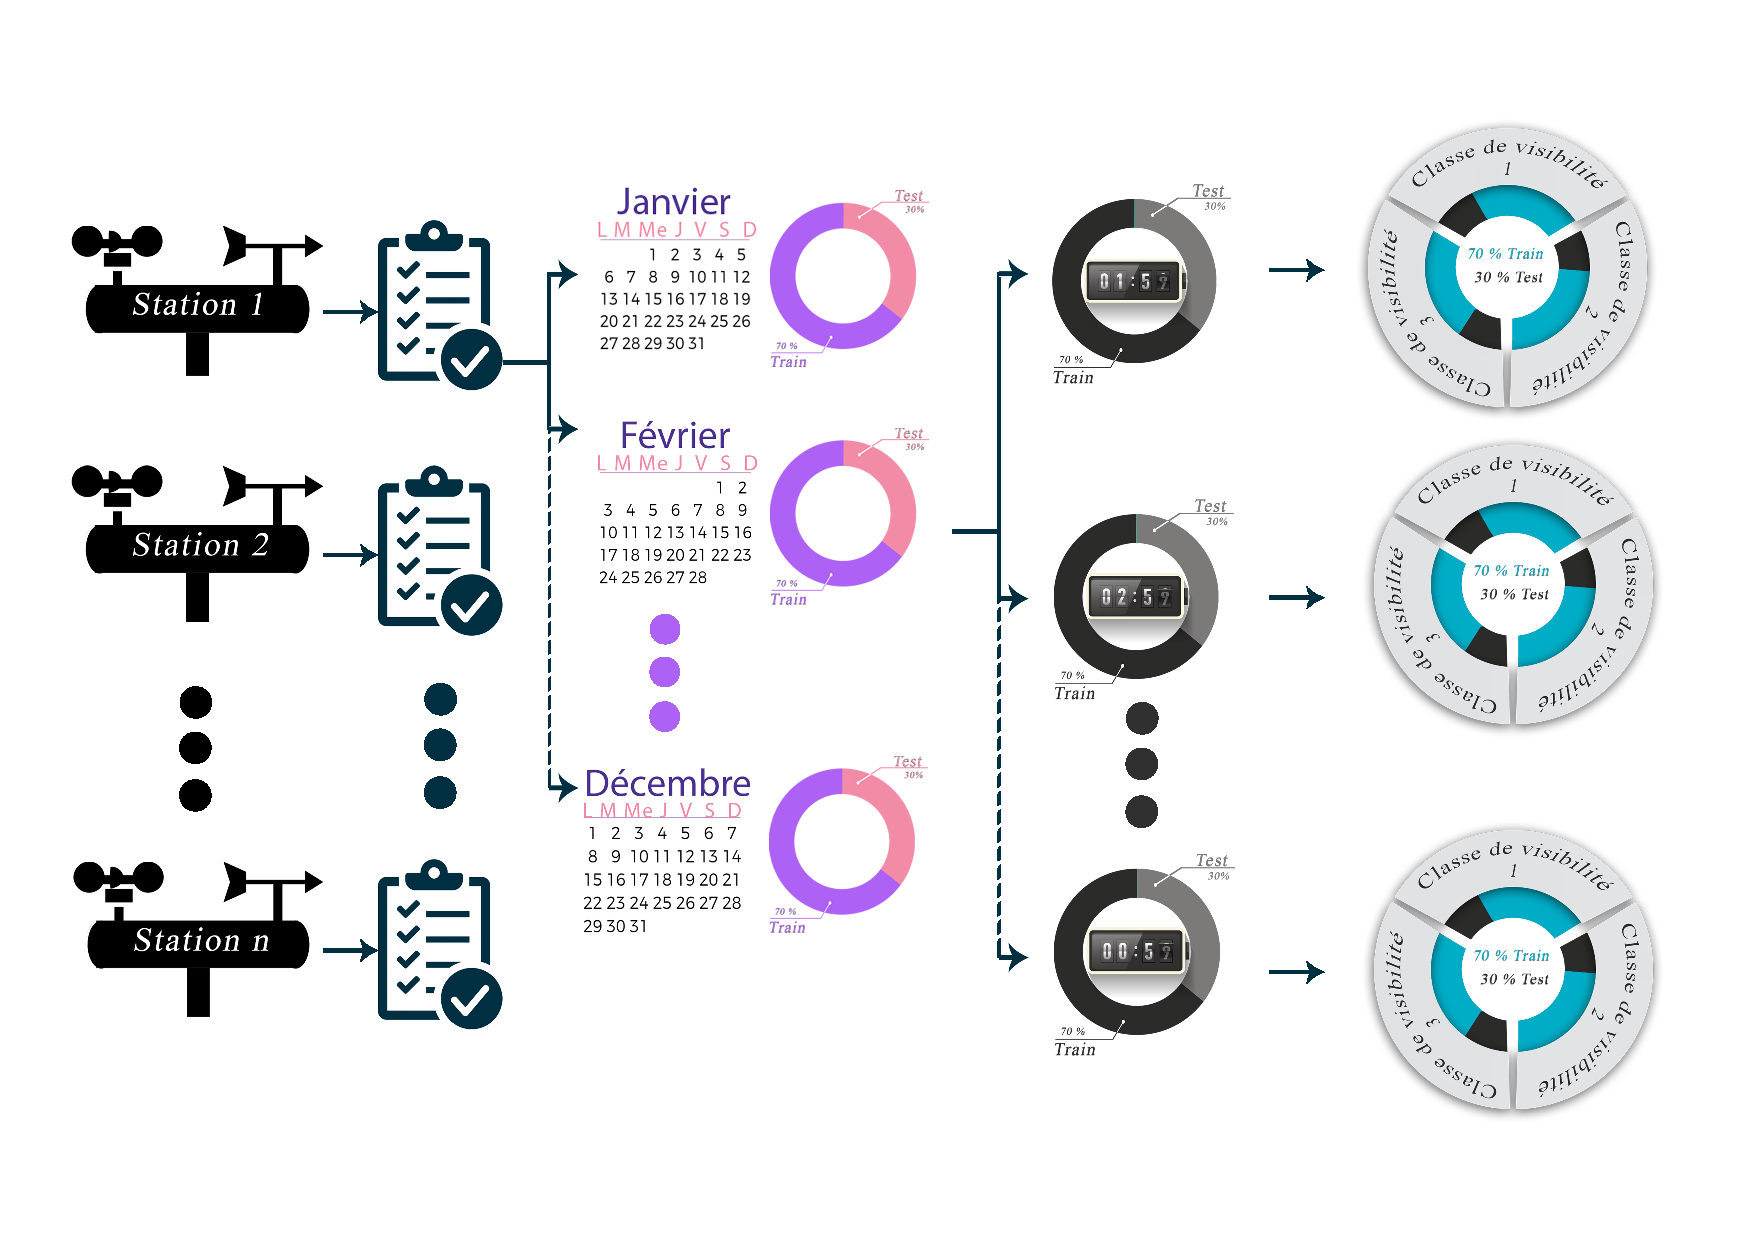
\includegraphics[width=23 cm, height= 14 cm]{img/data_prep.jpg}
\caption{La répartition des données}
\label{rep_donnees}
\end{figure}
\end{landscape}